\documentclass[]{article}
\usepackage{amsmath}
\usepackage{amsfonts}
\usepackage{amssymb}
\usepackage{amsthm}
\usepackage{cancel}
\usepackage{graphicx}
\usepackage{siunitx}
\usepackage{circuitikz}
\usepackage{pdfpages}
\usepackage{hyperref}

\renewcommand{\thesection}{\arabic{section}}
\renewcommand{\thesubsection}{\thesection.\alph{subsection}}
\renewcommand{\thesubsubsection}{\thesubsection.\roman{subsubsection}}

\newtheorem{genthm}{Theorem}

%opening
\title{EECS 16A HW07}
\author{Bryan Ngo}
\date{2019-10-16}

\begin{document}

\maketitle

\section{Circuit Analysis}

\subsection{}

\begin{circuitikz}[american]
	\draw (0, 3) to[V=\(\SI{5}{\volt}\), i>^=\(I_{V_s}\)] (0, 0);
	\draw (0, 3) to[R=\(\SI{2}{\ohm}\), i>^=\(I_{R_1}\), v_>=\(V_{R_1}\)] (3, 3);
	\draw (3, 3) to [R=\(\SI{2}{\ohm}\), i>^=\(I_{R_2}\), v_>=\(V_{R_2}\)] (6, 3);
	\draw (6, 3) to [I=\(\SI{2}{\ampere}\), l=\(V_{I_s}\)] (6, 0);
	\draw (6, 0) to[short] (0, 0);
	\draw (0, 0) node[ground]{};
	\draw (3, 3) to[R=\(\SI{4}{\ohm}\), i>^=\(I_{R_3}\), v=\(V_{R_3}\)] (3, 0);
\end{circuitikz}
There are 3 nodes to measure, \(U_1\) in the top left, \(U_2\) in the middle top, and \(U_3\) in the top right. There are also 5 currents: \(I_{R_1}, I_{R_2}, I_{R_3}, I_s,I_{V_s}\). KCL yields the equation
\begin{align}
	I_{V_s} + I_{R_1} &= 0 \\
	-I_{R_1} + I_{R_2} + I_{R_3} &= 0 \\
	-I_{R_2} + I_s &= 0
\end{align}
Plugging in our Ohm's Law relations, 
\begin{align}
	U_1 &= V_s \\
	I_s &= I_s \\
	U_1 - U_2 - I_{R_1} R_1 &= 0 \\
	U_2 - U_3 - I_{R_2} R_2 &= 0 \\
	U_2 - I_{R_3} R_3 &= 0
\end{align}
We can reduce this to a system of linear equations
\begin{equation}
	\begin{bmatrix}
	1 & 1 & 0 & 0 & 0 & 0 & 0 & 0 \\
	0 & -1 & 1 & 1 & 0 & 0 & 0 & 0 \\
	0 & 0 & -1 & 0 & 1 & 0 & 0 & 0 \\
	0 & 0 & 0 & 0 & 0 & 1 & 0 & 0 \\
	0 & 0 & 0 & 0 & 1 & 0 & 0 & 0 \\
	0 & -R_1 & 0 & 0 & 0 & 1 & -1 & 0 \\
	0 & 0 & -R_2 & 0 & 0 & 0 & 1 & -1 \\
	0 & 0 & 0 & -R_3 & 0 & 0 & 1 & 0
	\end{bmatrix}
	\begin{bmatrix}
	I_{V_s} \\
	I_{R_1} \\
	I_{R_2} \\
	I_{R_3} \\
	I_s \\
	U_1 \\
	U_2 \\
	U_3
	\end{bmatrix}
	=
	\begin{bmatrix}
	0 \\
	0 \\
	0 \\
	V_s \\
	I_2 \\
	0 \\
	0 \\
	0
	\end{bmatrix}
\end{equation}
Using a calculator, we attain the following values: 
\begin{equation}
	\mathbf{u} = \begin{bmatrix}
	-\frac{13}{6} \ \si{\ampere} \\
	\frac{13}{6} \ \si{\ampere} \\
	2 \ \si{\ampere} \\
	\frac{1}{6} \ \si{\ampere} \\
	2 \ \si{\ampere} \\
	5 \ \si{\volt} \\
	\frac{2}{3} \ \si{\volt} \\
	-\frac{10}{3} \ \si{\volt} \\
	\end{bmatrix}
\end{equation}

\subsection{}

\begin{center}
	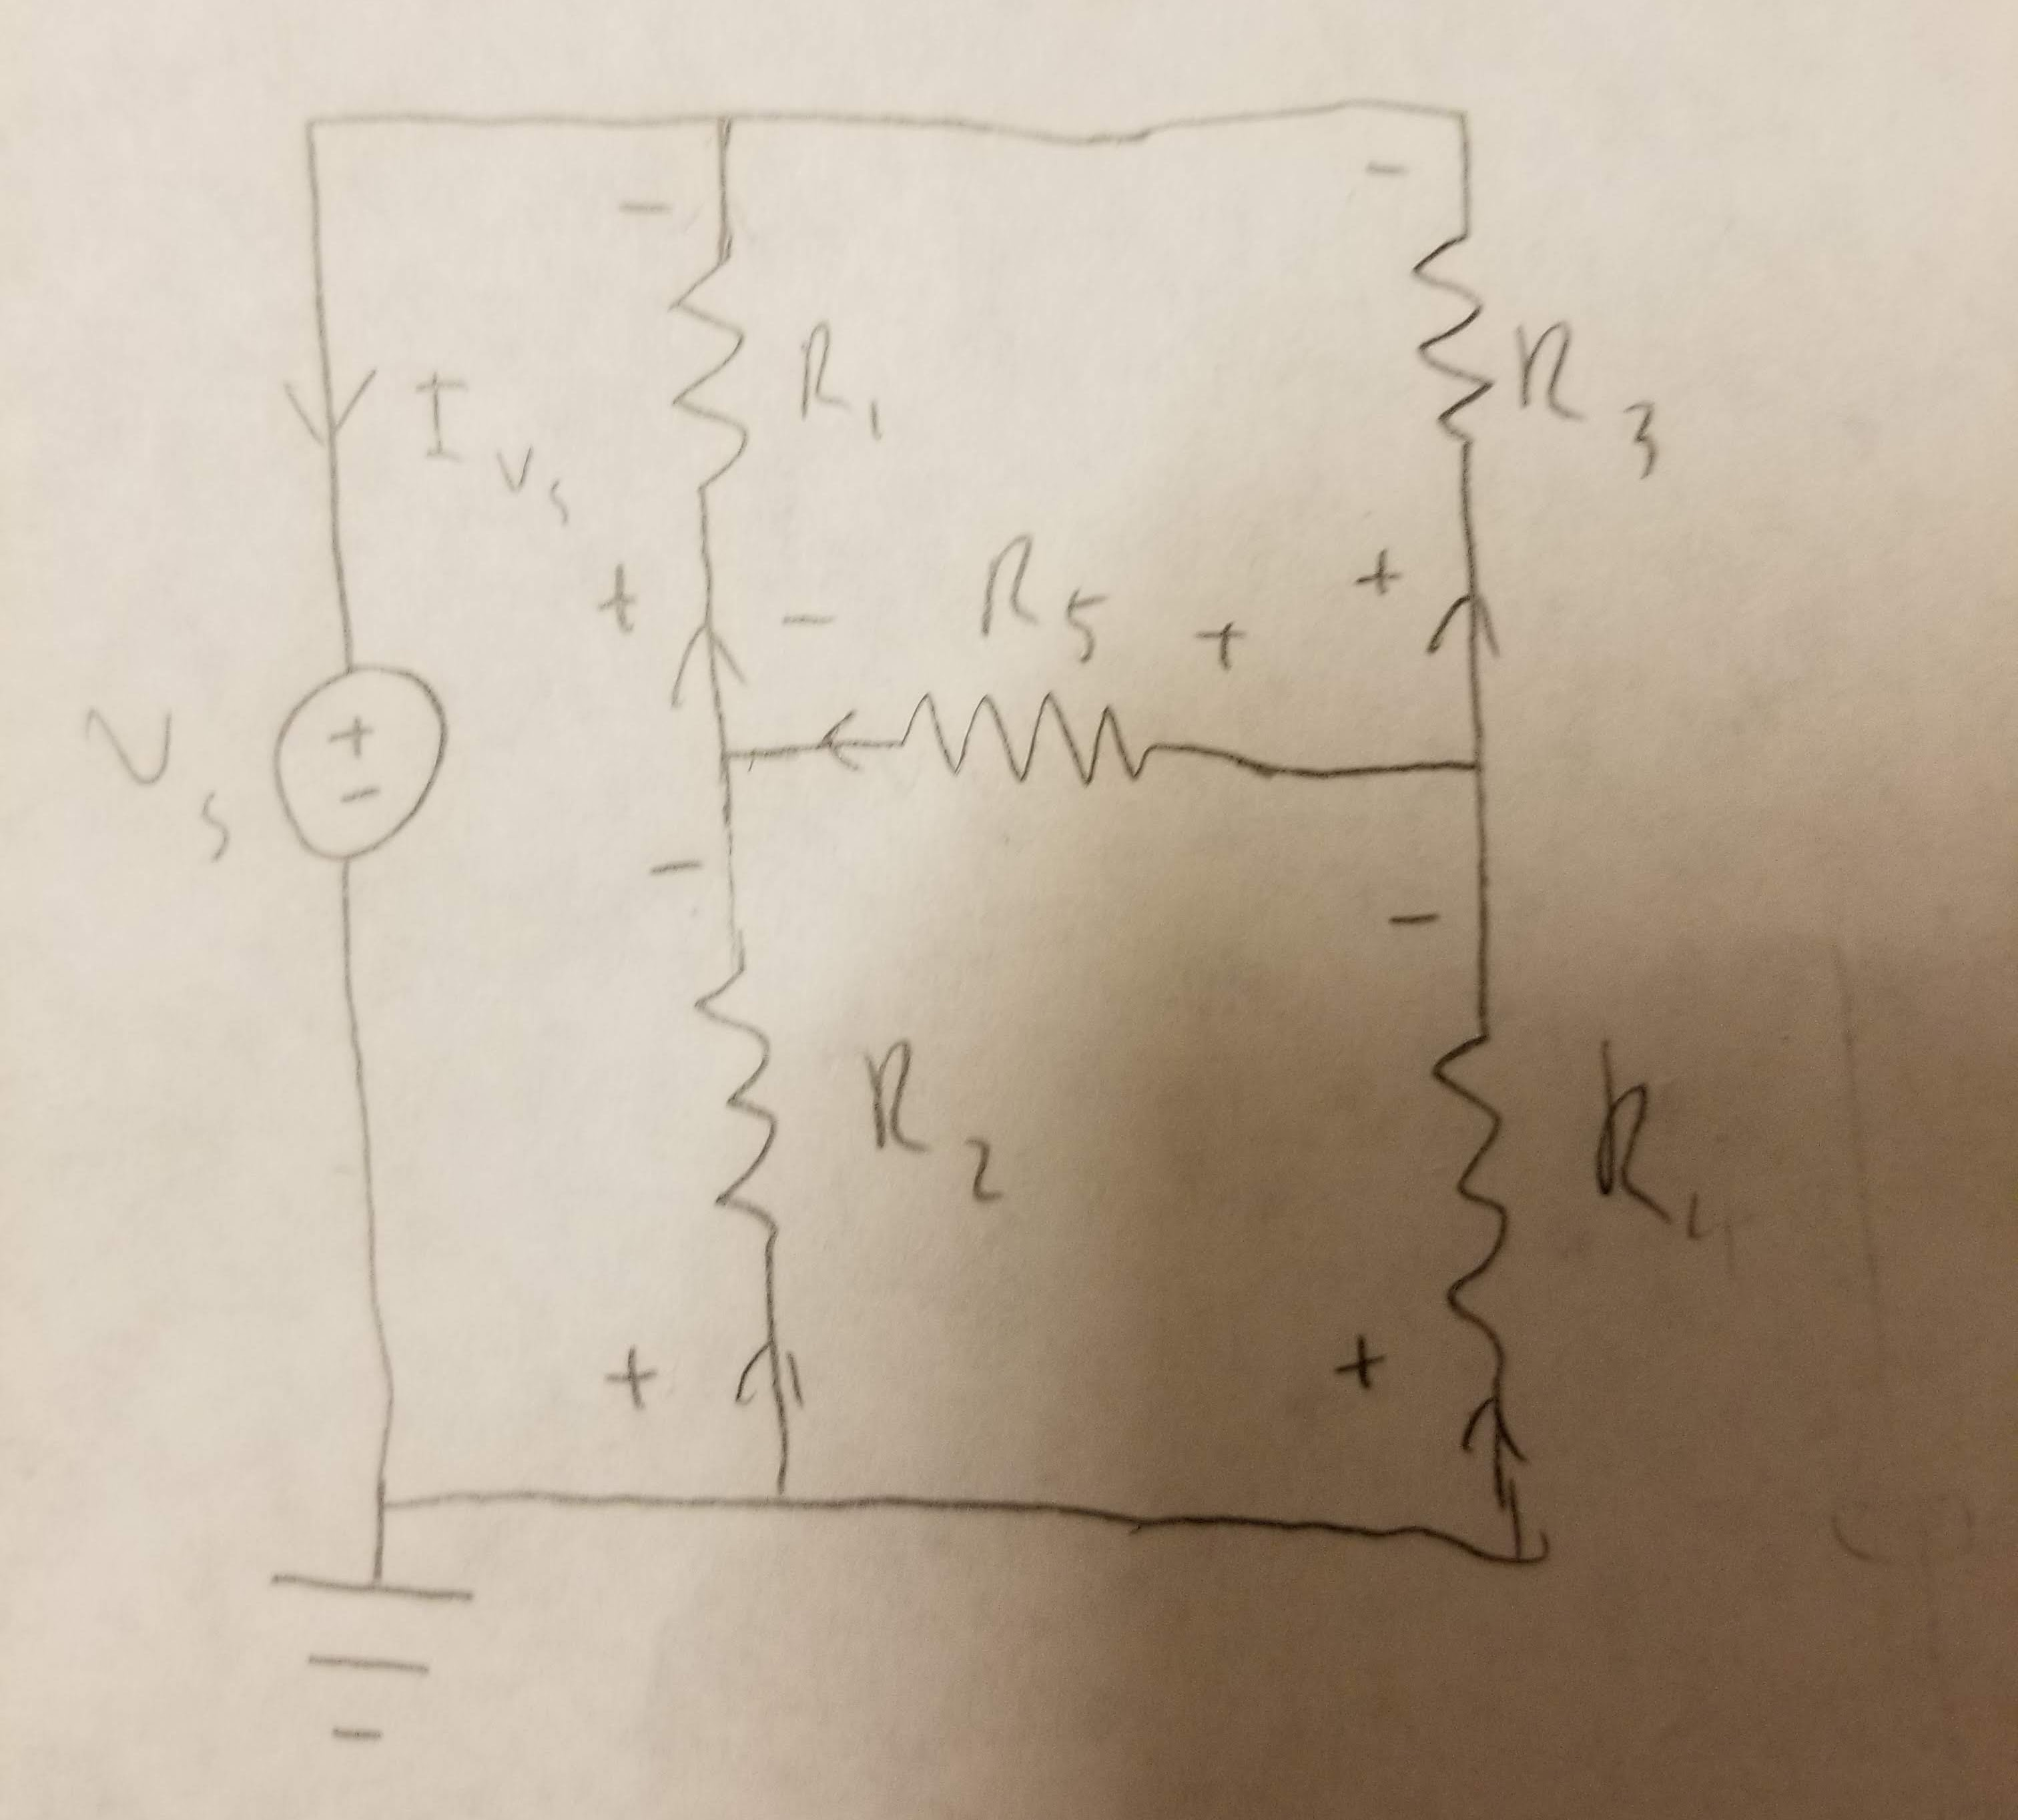
\includegraphics[width=0.7\linewidth]{20191018_214629}
\end{center}
Our KCL equations are 
\begin{align}
	I_{V_s} + I_{R_1} + I_{R_3} &= 0 \\
	-I_{R_1} + I_{R_2} + I_{R_5} &= 0 \\
	-I_{R_3} + I_{R_4} + I_{R_5} &= 0 \\
	U_1 &= V_s \\
	U_1 - U_2 - I_{R_1} R_1 &= 0 \\
	U_2 - I_{R_2} R_2 &= 0 \\
	U_1 - U_3 - I_{R_3} R_3 &= 0 \\
	U_3 - I_{R_4} R_4 &= 0 \\
	U_2 - U_3 - I_{R_5} R_5 &= 0
\end{align}
Converting to a matrix-vector multiplication, 
\begin{equation}
	\begin{bmatrix}
	1 & 1 & 0 & 1 & 0 & 0 & 0 & 0 & 0 \\
	0 & -1 & 1 & 0 & 0 & 1 & 0 & 0 & 0 \\
	0 & 0 & 0 & -1 & 1 & -1 & 0 & 0 & 0 \\
	0 & 0 & 0 & 0 & 0 & 0 & 1 & 0 & 0 \\
	0 & -R_1 & 0 & 0 & 0 & 0 & 1 & -1 & 0 \\
	0 & 0 & -R_2 & 0 & 0 & 0 & 0 & 1 & 0  \\
	0 & 0 & 0 & -R_3 & 0 & 0 & 1 & 0 & -1 \\
	0 & 0 & 0 & 0 & -R_4 & 0 & 0 & 0 & 1 \\
	0 & 0 & 0 & 0 & 0 & -R_5 & 0 & 1 & -1
	\end{bmatrix}
	\begin{bmatrix}
	I_{V_s} \\
	I_{R_1} \\
	I_{R_2} \\
	I_{R_3} \\
	I_{R_4} \\
	I_{R_5} \\
	U_1 \\
	U_2 \\
	U_3
	\end{bmatrix}
	=
	\begin{bmatrix}
	0 \\
	0 \\
	0 \\
	V_s \\
	0 \\
	0 \\
	0 \\
	0 \\
	0
	\end{bmatrix}
\end{equation}
Numerical Gaussian elimination gives us 
\begin{equation}
	\mathbf{u} = 
	\frac{1}{31}\begin{bmatrix}
	-74 \\
	53 \\
	51 \\
	21 \\
	23 \\
	2 \\
	155 \\
	102 \\
	92 \\
	\end{bmatrix}
\end{equation}

\section{1-D Resistive Touchscreen}

\subsection{}

\begin{circuitikz}[american]
	\draw (0, 3) to[V, i^=\(I_{V_s}\)] (0, 0);
	\draw (0, 3) to[short] (3, 3);
	\draw (3, 3) to[R=\(R\)] (3, 0);
	\draw (3, 0) to[short] (0, 0);
	\draw (0, 0) node[ground]{};
\end{circuitikz}

\subsection{}

Calculating the resistance of the touchscreen, 
\begin{equation}
	R = \frac{\rho_1 L}{W \cdot t} = \frac{\SI{0.5}{\ohm\meter} \cdot  \SI{80}{\milli\meter}}{\SI{50}{\milli\meter} \cdot \SI{1}{\milli\meter}} = \SI{800}{\ohm}
\end{equation}
Using Ohm's Law, 
\begin{equation}
	I_s = \frac{V_s}{R} = \frac{5}{800} = \SI{6.25}{\milli\ampere}
\end{equation}

\subsection{}

\begin{circuitikz}[american]
	\draw (0, 6) to[V, i^=\(I_{V_s}\)] (0, 0);
	\draw (0, 6) to[short] (3, 6);
	\draw (3, 6) to[R=\(R_1\)] (3, 3);
	\draw (3, 3) node[circ]{\ \(V_{12}\)};
	\draw (3, 3) to[R=\(R_2\)] (3, 0);
	\draw (3, 0) to[short] (0, 0);
	\draw (0, 0) node[ground]{};
\end{circuitikz}
The node voltage at \(V_{12}\) is 
\begin{equation}
	V_{12} = V_s \frac{y_2}{L} = \SI{3.75}{\volt}
\end{equation}

\subsection{}

The absolute difference between the voltages is 
\begin{equation}
	V_{ab} = V_s\left|\frac{y_1 - y_2}{L}\right| = \SI{1.875}{\volt}
\end{equation}

\subsection{}

Since this is a 1-D touchscreen, we can ignore the \(x\)-coordinate and only focus on the \(y\)-coordinate. 
Since the \(y\)-components are the same, their difference is \SI{0}{\meter} and thus so is the relative voltage of \SI{0}{\volt}. 

\subsection{}

Once more, we simply look at the \(y\)-coordinates. This leads us to say that it is the same relative voltage difference as the first one, or \SI{1.875}{\volt}. 

\subsection{}

\begin{circuitikz}[american]
	\draw (0, 3) to[V, i^=\(I_{V_s}\)] (0, 0);
	\draw (0, 3) to[short] (3, 3);
	\draw (3, 3) to[R=\(R_{\alpha}\)] (3, 0);
	\draw (3, 0) to[short] (0, 0);
	\draw (3, 3) to[short] (6, 3);
	\draw (6, 3) to[R=\(R_{\beta}\)] (6, 0);
	\draw (6, 0) to[short] (3, 0);
	\draw (0, 0) node[ground]{};
\end{circuitikz}

\subsection{}
Finding the resistance of \(R_{\beta}\), 
\begin{equation}
	R_{\beta} = \frac{\rho_2 L}{W_2 \cdot t} = \frac{\SI{0.4}{\ohm\meter} \cdot  \SI{70}{\milli\meter}}{\SI{50}{\milli\meter} \cdot \SI{1}{\milli\meter}} = \SI{457.14}{\ohm}
\end{equation}
We can find \(I_s\) by first finding the equivalent resistance, which is 
\begin{equation}
	R_{eq} = \frac{R_{\alpha} R_{\beta}}{R_{\alpha} + R_{\beta}} \approx \SI{291.0}{\ohm}
\end{equation}
Then, using Ohm's Law, 
\begin{equation}
	I_s = \frac{V_s}{R_{\alpha} \parallel R_{\beta}} \approx \SI{17.2}{\milli\ampere}
\end{equation}

\subsection{}

\begin{center}
	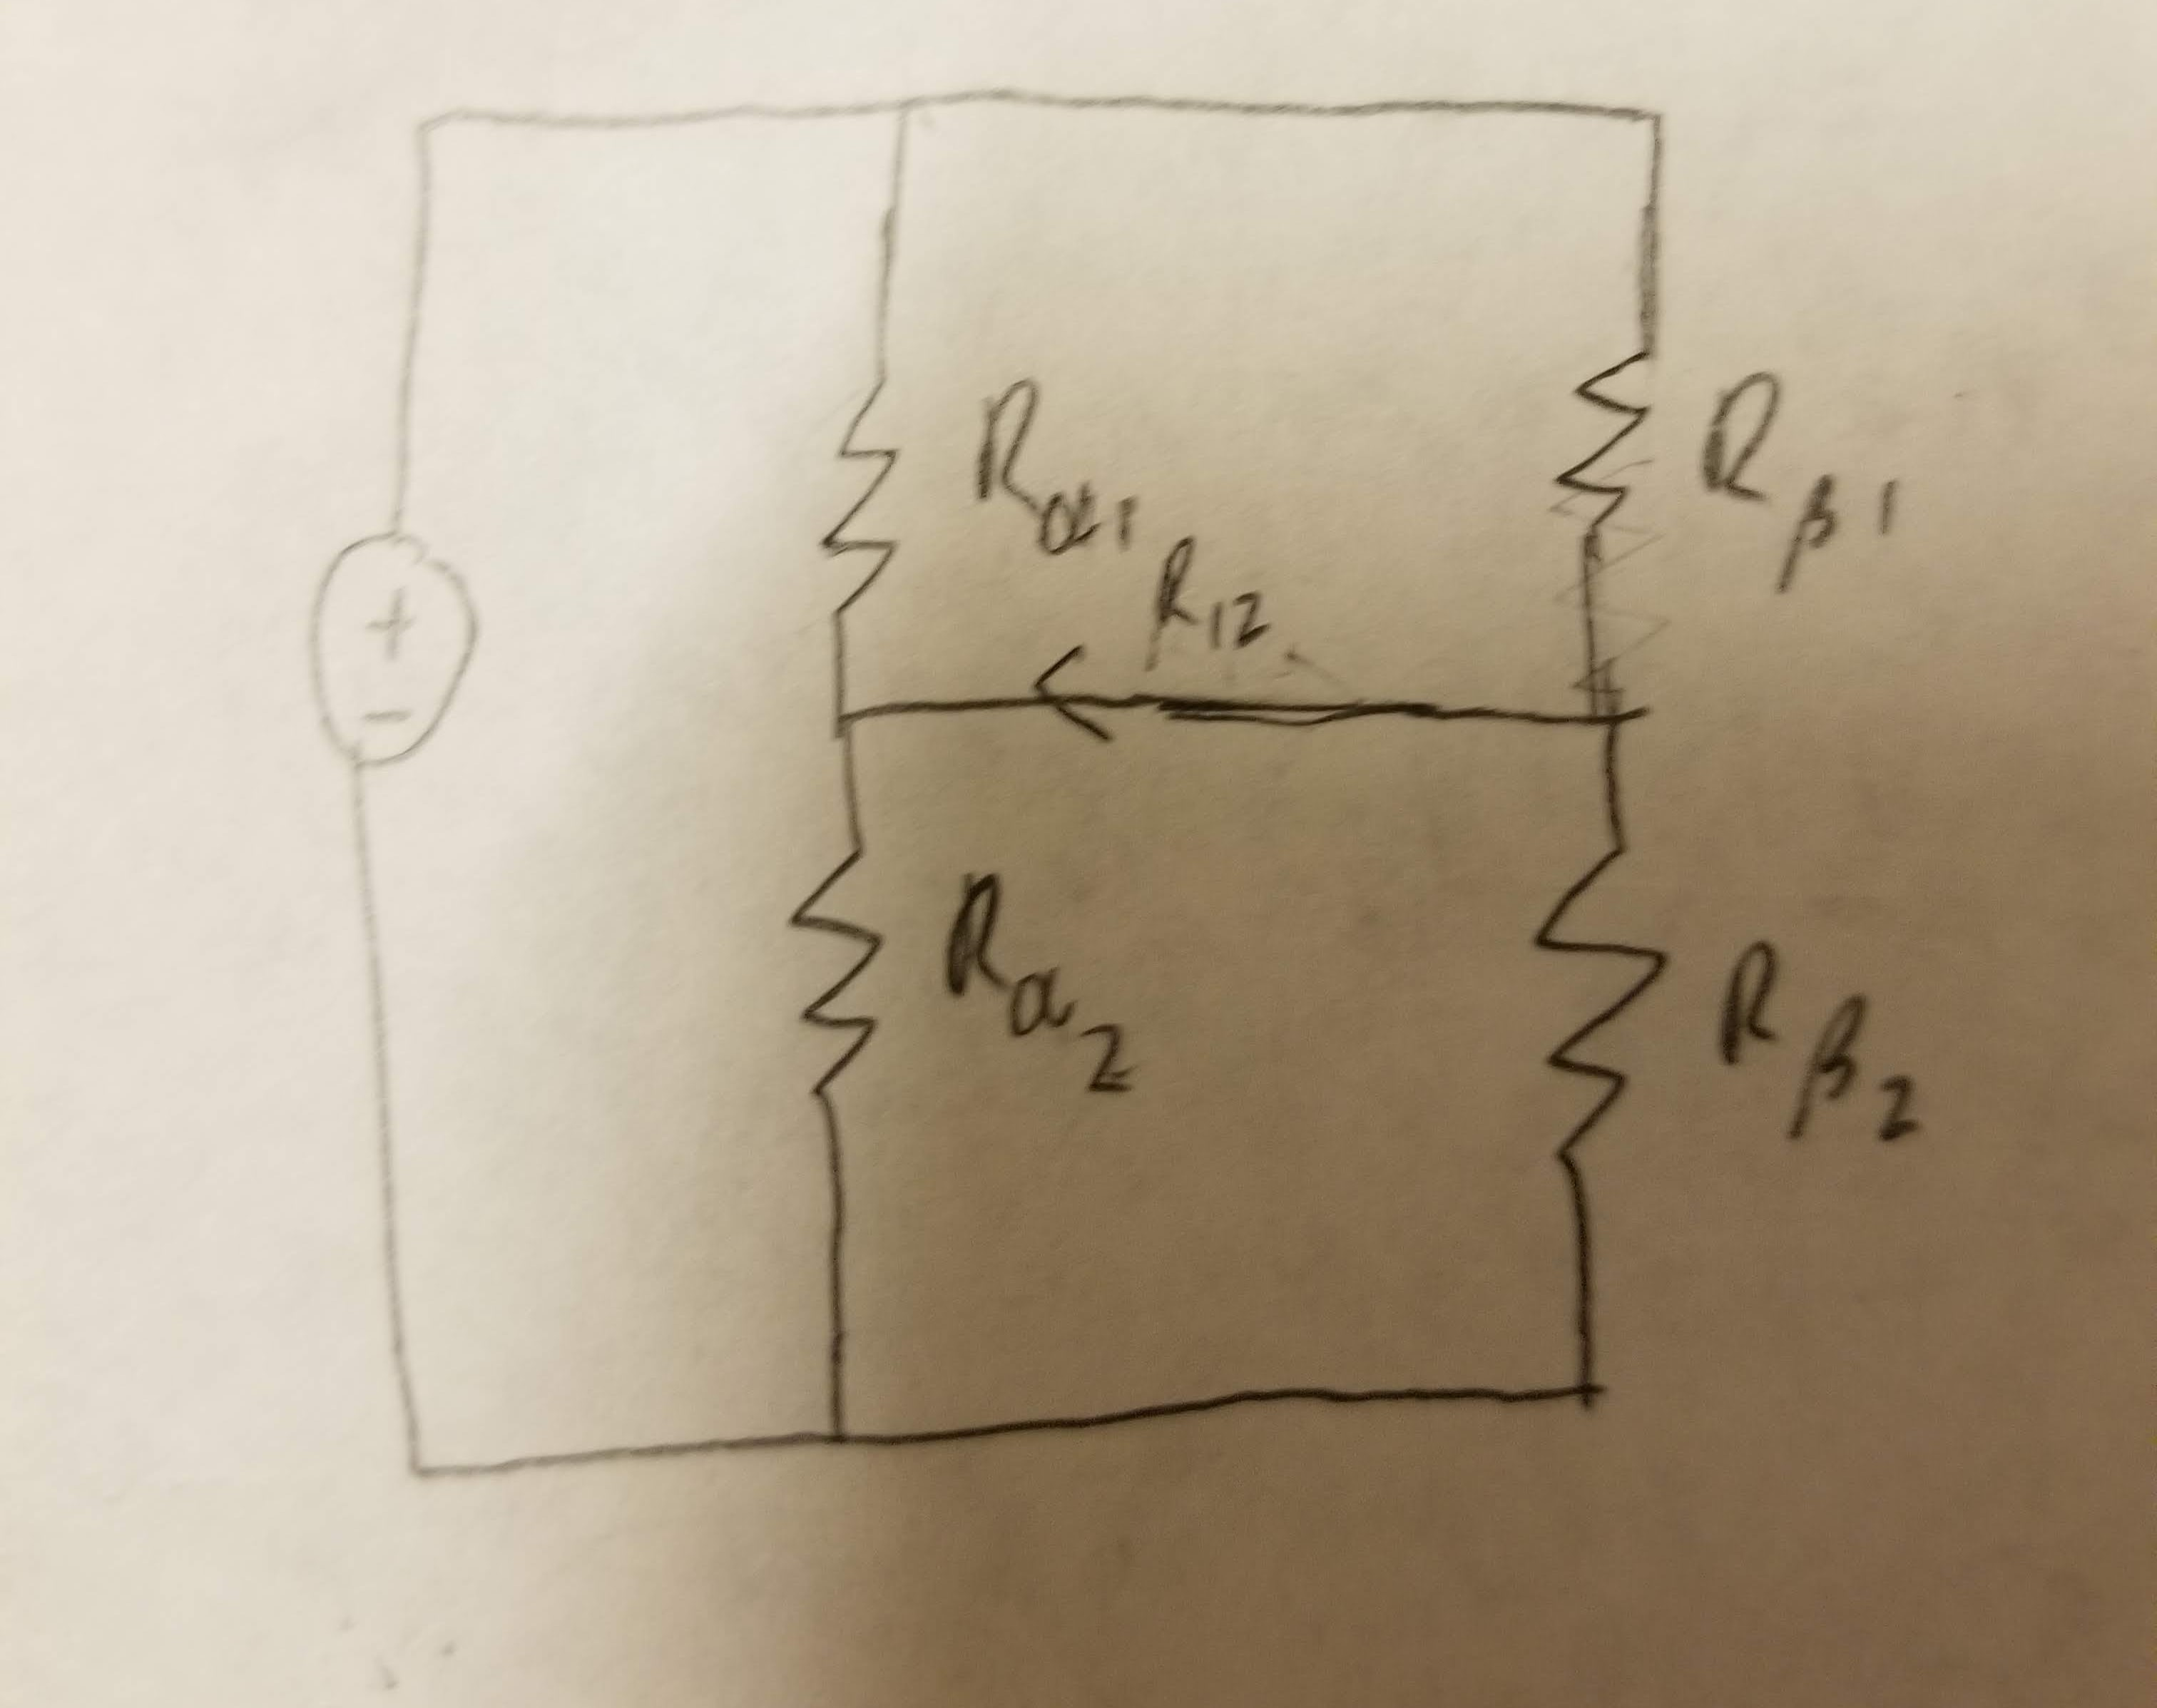
\includegraphics[width=0.7\linewidth]{20191018_214635}
\end{center}
We can reuse the matrix from 1.b, since the circuit topology is the same. 
This time, however, we plug in different values of resistances: 
\begin{align}
	R_{\alpha 1} &= \frac{\rho_1 (L - y_2)}{W_1 \cdot t} = \SI{200}{\ohm} \\
	R_{\alpha 2} &= \frac{\rho_1 (y_2)}{W_1 \cdot t} = \SI{600}{\ohm} \\
	R_{\beta 1} &= \frac{\rho_2 (L - y_2)}{W_2 \cdot t} \approx \SI{114.29}{\ohm} \\
	R_{\beta 2} &= \frac{\rho_2 y_2}{W_2 \cdot t} \approx \SI{342.86}{\ohm} \\
\end{align}
\(R_5\) is shorted and thus has zero resistance because it is simply a wire. 
Plugging into the matrix
\begin{equation}
	\begin{bmatrix}
	1 & 1 & 0 & 1 & 0 & 0 & 0 & 0 & 0 \\
	0 & -1 & 1 & 0 & 0 & 1 & 0 & 0 & 0 \\
	0 & 0 & 0 & -1 & 1 & -1 & 0 & 0 & 0 \\
	0 & 0 & 0 & 0 & 0 & 0 & 1 & 0 & 0 \\
	0 & -R_{\alpha 1} & 0 & 0 & 0 & 0 & 1 & -1 & 0 \\
	0 & 0 & -R_{\alpha 2} & 0 & 0 & 0 & 0 & 1 & 0  \\
	0 & 0 & 0 & -R_{\beta 1} & 0 & 0 & 1 & 0 & -1 \\
	0 & 0 & 0 & 0 & -R_{\alpha 2} & 0 & 0 & 0 & 1 \\
	0 & 0 & 0 & 0 & 0 & 0 & 0 & 1 & -1
	\end{bmatrix}
	\begin{bmatrix}
	I_{V_s} \\
	I_{R_1} \\
	I_{R_2} \\
	I_{R_3} \\
	I_{R_4} \\
	I_{R_5} \\
	U_1 \\
	U_2 \\
	U_3
	\end{bmatrix}
	=
	\begin{bmatrix}
	0 \\
	0 \\
	0 \\
	V_s \\
	0 \\
	0 \\
	0 \\
	0 \\
	0
	\end{bmatrix}
\end{equation}
Gaussian elimination yields an \(I_{R_5}\) of \SI{-2d-15}{\ampere}. 

\section{Volt and Ammeter}

\subsection{}

\begin{center}
	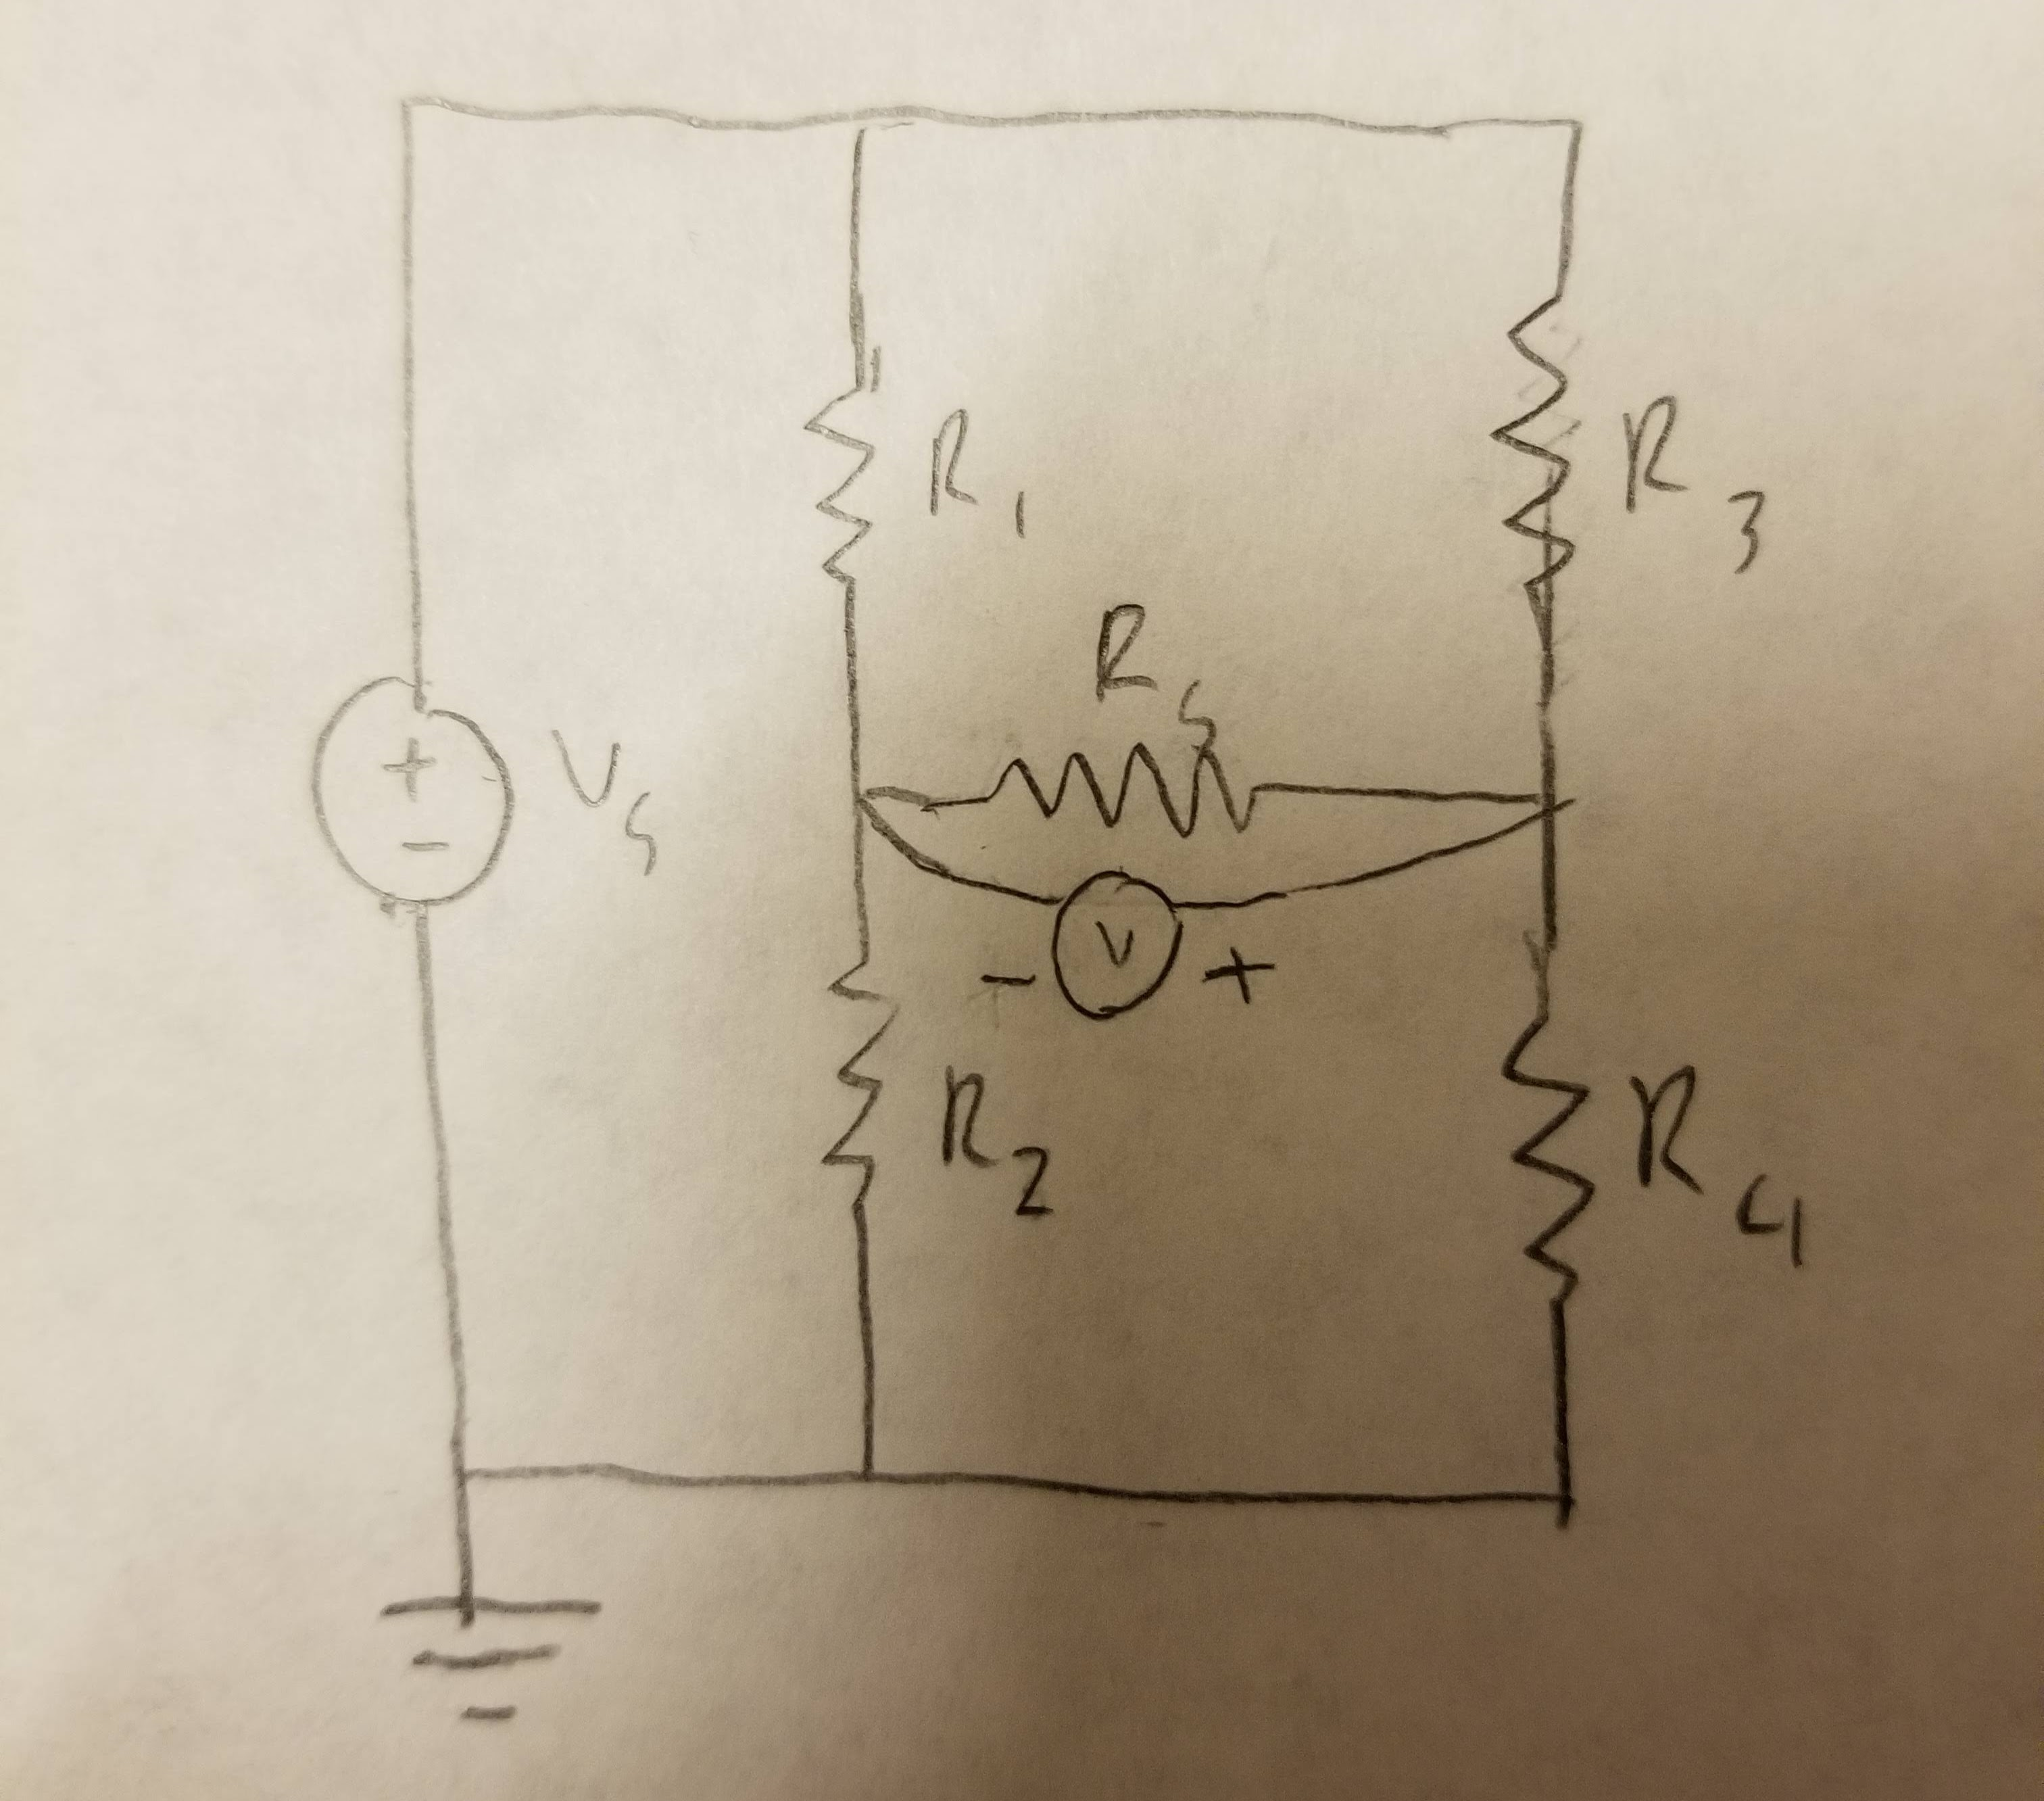
\includegraphics[width=0.7\linewidth]{20191018_214624}
\end{center}
The result can be calculated from Ohm's Law and the result from 1.b. 
Since all the resistances are 1000 times greater, the currents are 1000 times smaller, but the node voltages stay the same. Thus, the voltage measured is just the difference of the node voltages \(U_2, U_3\): 
\begin{equation}
	V_{ab} = U_2 - U_3 = \frac{10}{31} \ \si{\volt}
\end{equation}

\subsection{}

Since an ideal ammeter is a \SI{0}{\ohm} resistor, it shorts \(R_5\). 
This means that there is no potential difference across it, and \(V_{ab} = \SI{0}{\volt}\). 

\subsection{}

\begin{center}
	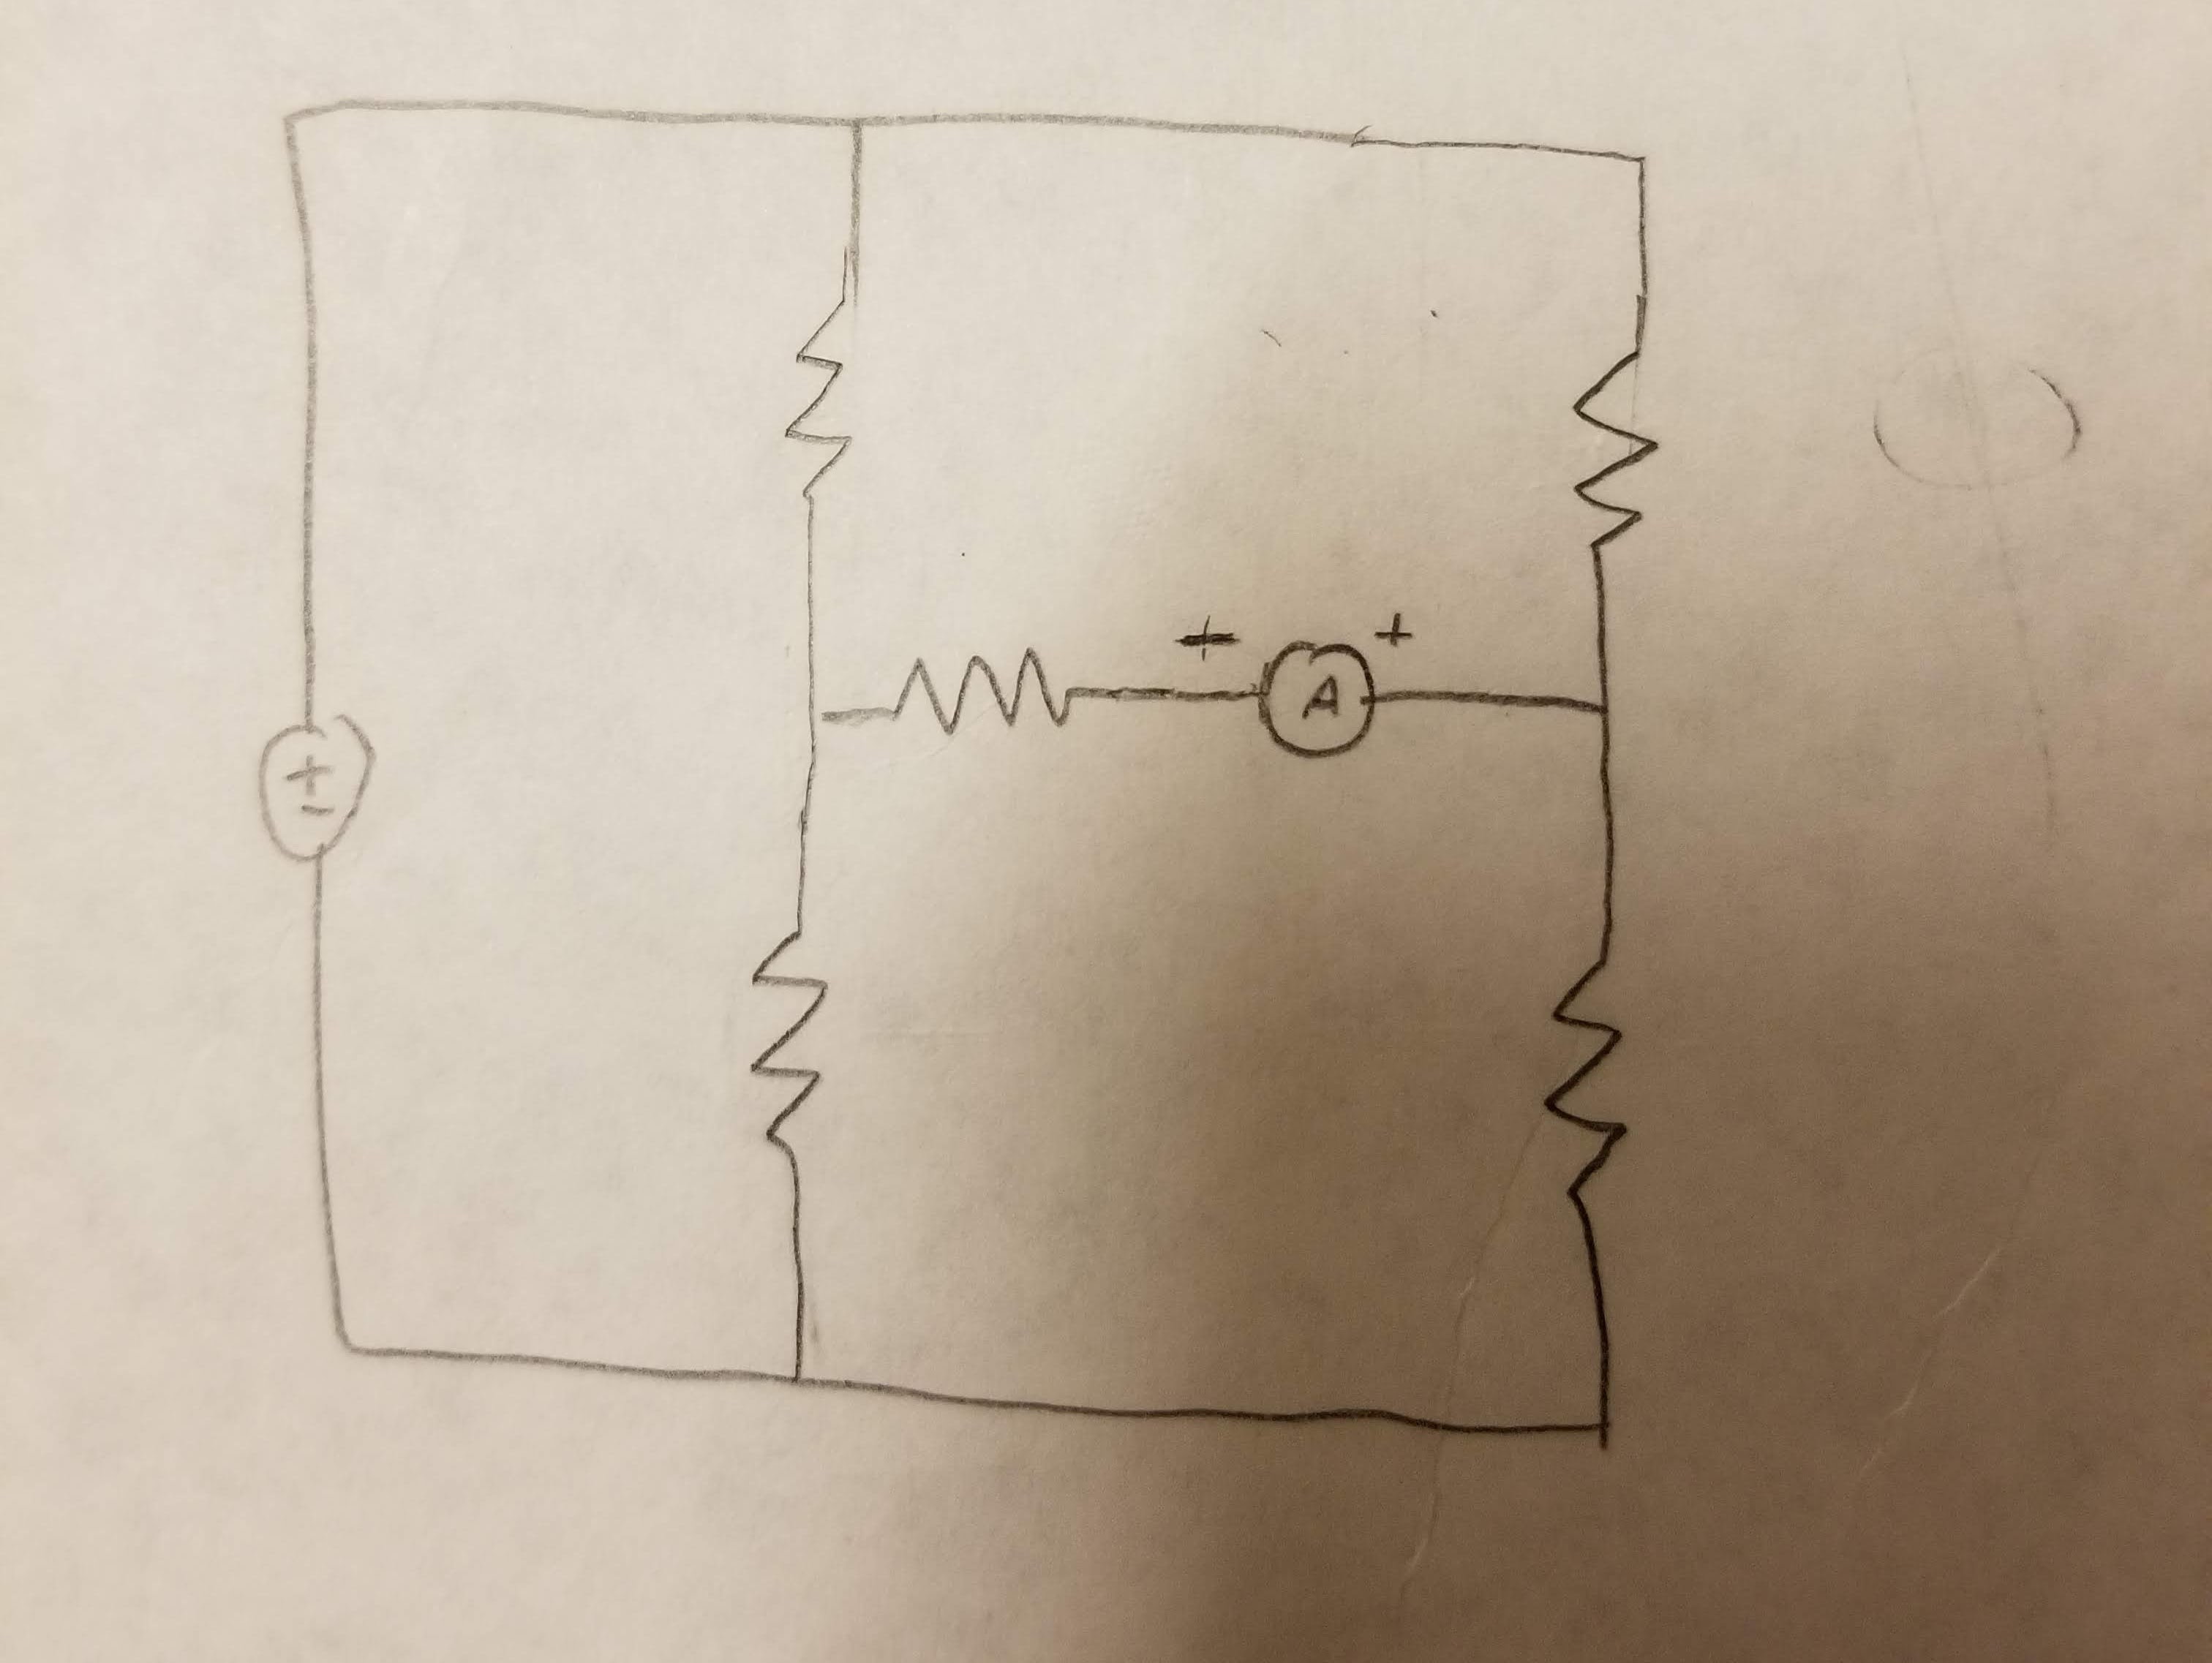
\includegraphics[width=0.7\linewidth]{20191018_214633}
\end{center}
Since the circuit has 1000 times the resistance, the current through \(R_5\) is simply 1000 times less than the current going through \(R_5\) in 1.b, which is \(I_{R_5} = 2/31 \ \si{\milli\ampere}\). 

\subsection{}

Connecting a voltmeter in series with \(R_5\) makes it effectively an open circuit, so no current can flow. \(I_{R_5} = \SI{0}{\ampere}\). 

\section{Fruity Fred}

\subsection{}

\begin{equation}
	R_{ab} = 2\frac{\rho (L - kF)}{A_c}
\end{equation}
The factor of 2 appears because there are 2 resistors in series, so we simply add them up. 

\subsection{}

\begin{circuitikz}[american]
	\draw (0, 0) to[V_=\(V_s\), i=\(I_s\)] (3, 0);
	\draw (3, 0) to[R=\(M_1\), *-*] (3, 3);
	\draw (3, 3) to[short] (0, 3);
	\draw (0, 3) to[R=\(M_2\)] (0, 0);
	\draw (3, 0) to[short] (5, 0);
	\draw (5, 0) to[voltmeter] (5, 3);
	\draw (5, 3) to[short] (3, 3);
\end{circuitikz}
The voltage is measured at the two terminal points. 
We can measure the voltage simply by leveraging KVL: 
\begin{equation}
	V_s - I M_1 - I M_2 = 0
\end{equation}
Where \(I\) is the current going through the circuit. 
	Plugging in the resistance values found in the last question, 
\begin{equation}
	V_s - 2I\frac{\rho (L - kF)}{A_c} = 0
\end{equation}

\section{Homework Process and Study Group}

I worked with Alfred Quan (SID: 3034658446). 

\newpage

%\includepdf[pages=-]{prob*.pdf}

\end{document}
